\documentclass[11pt,a4paper]{article}

% Packages
\usepackage[utf8]{inputenc}
\usepackage[T1]{fontenc}
\usepackage{amsmath,amssymb}
\usepackage{graphicx}
\usepackage{booktabs}
\usepackage{hyperref}
\usepackage[margin=1in]{geometry}
\usepackage{caption}
\usepackage{subcaption}
\usepackage{listings}
\usepackage{xcolor}
\usepackage{float}

\lstset{
    basicstyle=\ttfamily\small,
    breaklines=true,
    frame=single,
    backgroundcolor=\color{gray!10},
}

\title{SL-GPS Validation Report:\\DMM (CH$_3$OCH$_2$OCH$_3$) Mechanism Reduction\\via Supervised Learning --- PODE-1}
\author{SL-GPS Automated Validation Framework}
\date{\today}

\begin{document}

\maketitle

\begin{abstract}
This report presents the validation of the Supervised Learning -- Global Pathway Selection (SL-GPS) method for adaptive chemical mechanism reduction applied to dimethoxymethane (DMM, CH$_3$OCH$_2$OCH$_3$) combustion using the PODE-1 mechanism (586 species, 3091 reactions). DMM is a polyoxymethylene dimethyl ether (PODE$_1$) of interest as a soot-free diesel surrogate. The validation campaign spans 35 cases covering 700--1600~K, 1--20~atm, and $\phi$ 0.5--1.6, with baseline and expanded test matrices including NTC regime probes and extrapolation boundary tests.
\end{abstract}

\tableofcontents
\newpage

% =============================================================================
\section{Introduction}
% =============================================================================

The SL-GPS method trains neural networks on Global Pathway Selection (GPS) data to dynamically predict which chemical species are important during combustion simulations. This report validates SL-GPS on the PODE-1 mechanism for dimethoxymethane (DMM, CH$_3$OCH$_2$OCH$_3$, C$_3$H$_8$O$_2$, MW=76.09), a key polyoxymethylene dimethyl ether surrogate.

\subsection{Mechanism Overview}

\begin{table}[H]
\centering
\caption{PODE-1 mechanism summary.}
\label{tab:mech}
\begin{tabular}{ll}
\toprule
\textbf{Property} & \textbf{Value} \\
\midrule
Name & PODE-1 (Labb\'{e} Lab) \\
Species & 586 \\
Reactions & 3091 \\
Target fuels & DMM / oxygenated C$_1$--C$_4$ \\
Format & Cantera YAML (from CHEMKIN) \\
\bottomrule
\end{tabular}
\end{table}

% =============================================================================
\section{Methodology}
\label{sec:methodology}
% =============================================================================

\subsection{SL-GPS Pipeline}

\begin{enumerate}
    \item \textbf{Data generation:} Run $N$ autoignition simulations with randomized initial conditions ($T$, $P$, $\phi$). At each timestep interval, apply GPS ($\alpha = 0.001$) to label which species are important.
    \item \textbf{ANN training:} Train an ensemble of neural networks on the GPS-labeled data. Select the best model by validation loss.
    \item \textbf{Validation:} Run new autoignition cases with the detailed mechanism and simultaneously with SL-GPS (ANN-guided reduction). Compare temperature, HRR, species profiles, and ignition delay.
\end{enumerate}

\subsection{Neural Network Architecture}

\begin{itemize}
    \item \textbf{Input:} temperature, pressure, and 14 selected species mole fractions (normalized via MinMaxScaler)
    \item \textbf{Hidden layers:} 2 fully-connected layers $\times$ 32 neurons with ReLU activation
    \item \textbf{Output:} sigmoid activation (one output per variable species)
    \item \textbf{Loss:} binary cross-entropy; \textbf{Optimizer:} Adam
    \item \textbf{Training:} parallel ensemble (8--12 seeds), best selected by validation loss
    \item \textbf{Early stopping:} patience = 30 epochs, max = 200 epochs
\end{itemize}

% =============================================================================
\section{DMM --- PODE-1}
\label{sec:dmm}
% =============================================================================

\subsection{Training Configuration}

\begin{table}[H]
\centering
\caption{DMM training configuration.}
\label{tab:dmm_config}
\begin{tabular}{ll}
\toprule
\textbf{Parameter} & \textbf{Value} \\
\midrule
\multicolumn{2}{l}{\textit{Mechanism}} \\
\quad Mechanism & PODE-1 (Labb\'{e} Lab) \\
\quad Species / Reactions & 586 / 3091 \\
\midrule
\multicolumn{2}{l}{\textit{Data Generation}} \\
\quad Training cases & 15 (parallel execution) \\
\quad Temperature range & 800--1600~K (uniform) \\
\quad Pressure range & 1--20~atm (log-uniform) \\
\quad Equivalence ratio $\phi$ & 0.7--1.4 (uniform) \\
\quad GPS $\alpha$ & 0.001 \\
\midrule
\multicolumn{2}{l}{\textit{ANN Training}} \\
\quad Input features & $T$, $P$ + 14 species mole fractions \\
\quad Architecture & 2 hidden layers $\times$ 32 neurons \\
\quad Ensemble size & 8 parallel trainings \\
\quad Max epochs / Early stopping & 200 / patience 30 \\
\bottomrule
\end{tabular}
\end{table}

\textbf{Input species (ANN features):} CH$_3$OCH$_2$OCH$_3$, O$_2$, H$_2$O, CO$_2$, CO, OH, H, H$_2$, CH$_4$, CH$_2$O, CH$_3$OH, HO$_2$, CH$_3$O, HCO

\subsection{Validation Cases}

\begin{table}[H]
\centering
\caption{DMM baseline validation conditions.}
\label{tab:dmm_cases}
\begin{tabular}{lcccc}
\toprule
\textbf{Case} & \textbf{$T_0$ (K)} & \textbf{$P$ (atm)} & \textbf{$\phi$} & \textbf{$t_{\text{end}}$ (s)} \\
\midrule
T1000\_P1 & 1000 & 1 & 1.0 & 0.2 \\
T1200\_P1 & 1200 & 1 & 1.0 & 0.02 \\
T1200\_P10 & 1200 & 10 & 1.0 & 0.005 \\
T1500\_P1 & 1500 & 1 & 1.0 & 0.005 \\
\midrule
\multicolumn{5}{c}{\textit{Extended cases}} \\
\midrule
T800\_P20 & 800 & 20 & 1.0 & 0.5 \\
T900\_P10 & 900 & 10 & 1.0 & 0.1 \\
T1100\_P1\_rich & 1100 & 1 & 1.3 & 0.05 \\
T1400\_P5\_lean & 1400 & 5 & 0.7 & 0.005 \\
\bottomrule
\end{tabular}
\end{table}

\subsection{Results}

\begin{table}[H]
\centering
\caption{DMM validation results: all 8 cases pass ($<10\%$ ignition delay error).}
\label{tab:dmm_results}
\begin{tabular}{lccccccc}
\toprule
\textbf{Case} & \textbf{$T_0$ (K)} & \textbf{$P$ (atm)} & \textbf{$\phi$} & \textbf{$\tau_{\text{det}}$ (ms)} & \textbf{$\tau_{\text{SL}}$ (ms)} & \textbf{Error (\%)} & \textbf{Avg Sp} \\
\midrule
T1000\_P1      & 1000 &  1.0 & 1.0 & 33.570 & 33.467 & 0.3 & 35 \\
T1200\_P1      & 1200 &  1.0 & 1.0 &  0.665 &  0.679 & 2.1 & 27 \\
T1200\_P10     & 1200 & 10.0 & 1.0 &  0.184 &  0.183 & 0.8 & 30 \\
T1500\_P1      & 1500 &  1.0 & 1.0 &  0.032 &  0.033 & 2.3 & 26 \\
T800\_P20      &  800 & 20.0 & 1.0 & 28.373 & 28.379 & 0.0 & 36 \\
T900\_P10      &  900 & 10.0 & 1.0 & 13.858 & 13.827 & 0.2 & 38 \\
T1100\_P1\_rich & 1100 &  1.0 & 1.3 &  3.520 &  3.634 & 3.2 & 31 \\
T1400\_P5\_lean & 1400 &  5.0 & 0.7 &  0.026 &  0.027 & 1.9 & 34 \\
\midrule
\multicolumn{6}{l}{\textbf{Mean ignition delay error}} & \textbf{1.4\%} & \\
\multicolumn{6}{l}{\textbf{Mean species count / reduction}} & & \textbf{32 / 95\%} \\
\bottomrule
\end{tabular}
\end{table}

\begin{figure}[H]
\centering
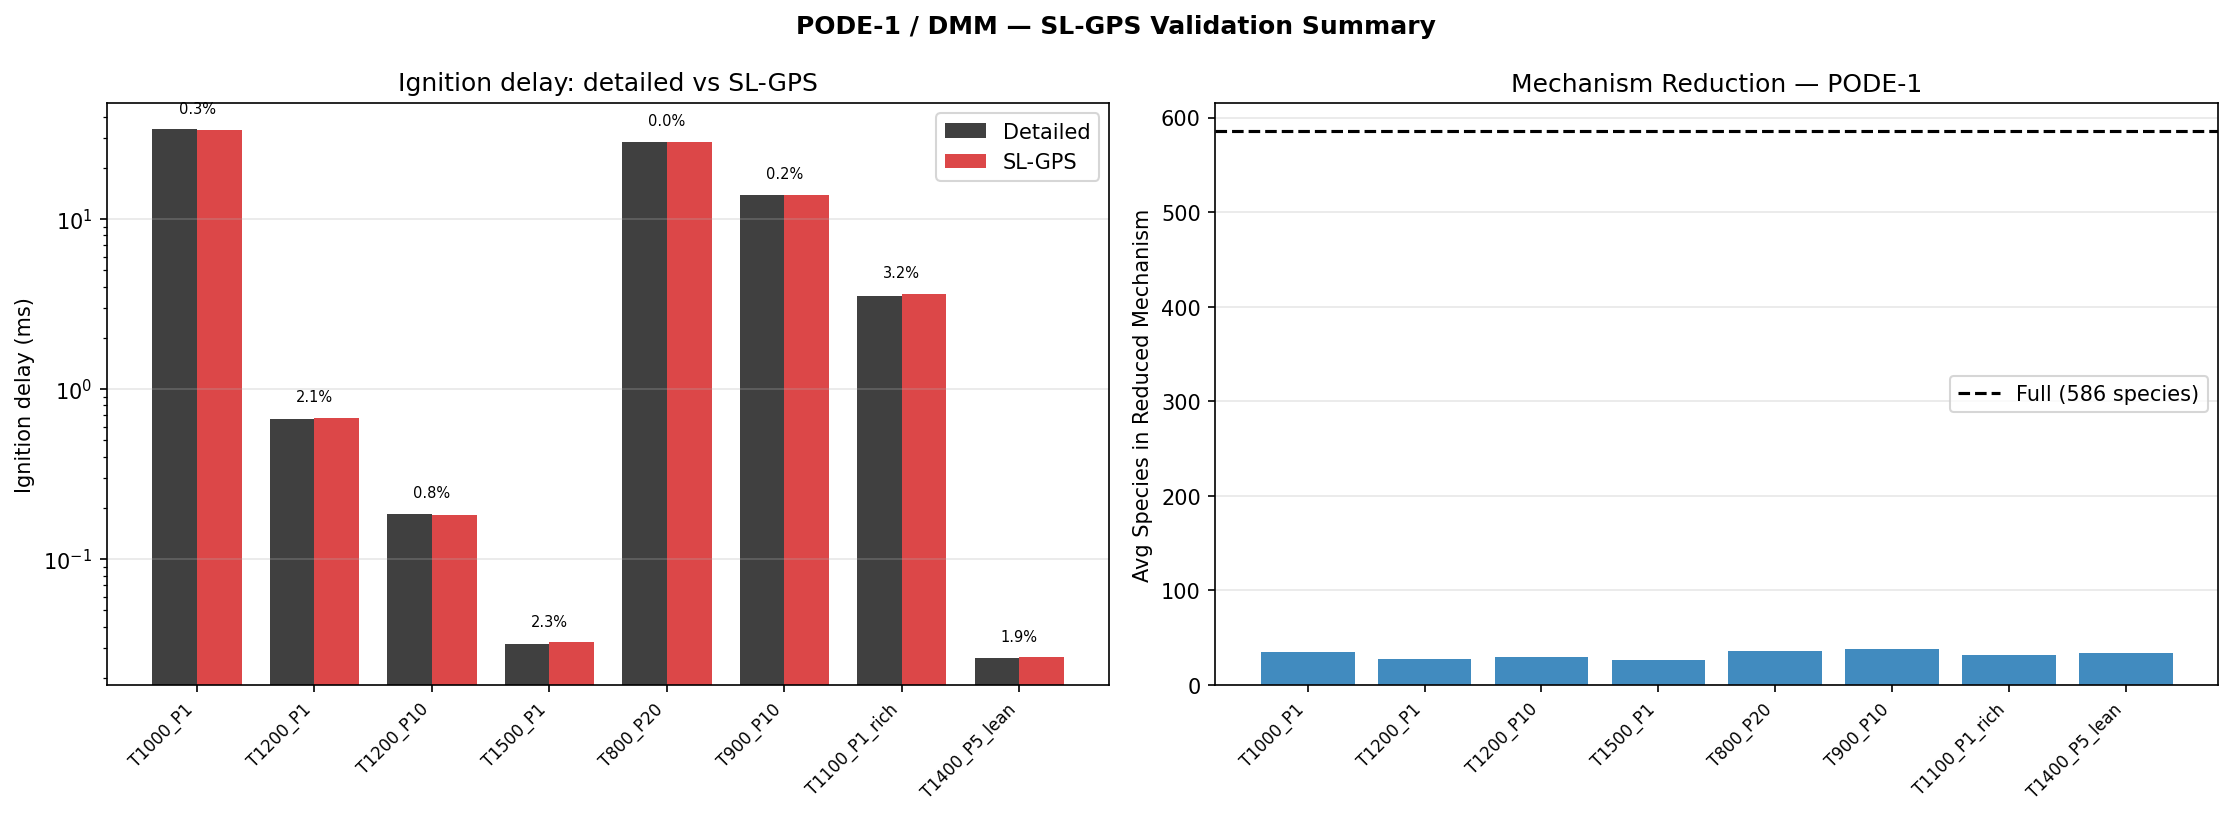
\includegraphics[width=0.95\textwidth]{results/dmm/DMM_summary.png}
\caption{DMM validation summary: ignition delay comparison (left) and mechanism reduction (right). All 8 cases pass with mean error 1.4\% and 95\% mean reduction (32 of 586 species).}
\label{fig:dmm_summary}
\end{figure}

\subsection{Individual Case Results}

\begin{figure}[H]
    \centering
    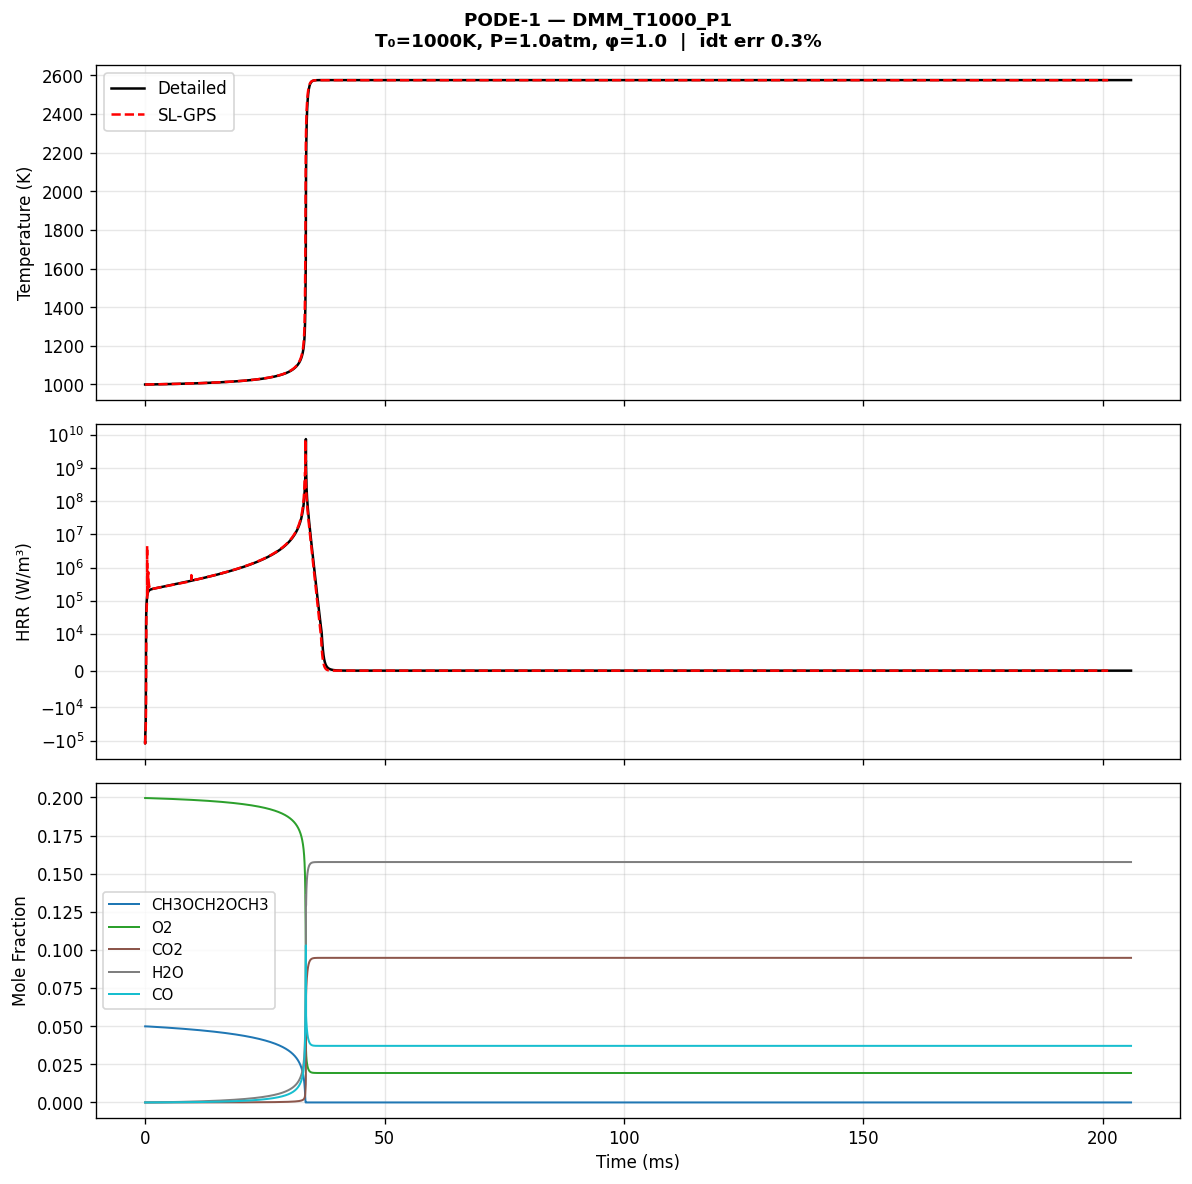
\includegraphics[width=0.95\textwidth]{results/dmm/DMM_T1000_P1.png}
    \caption{DMM: $T_0=1000$~K, $P=1$~atm, $\phi=1.0$. Ignition delay error: 0.3\%.}
\end{figure}

\begin{figure}[H]
    \centering
    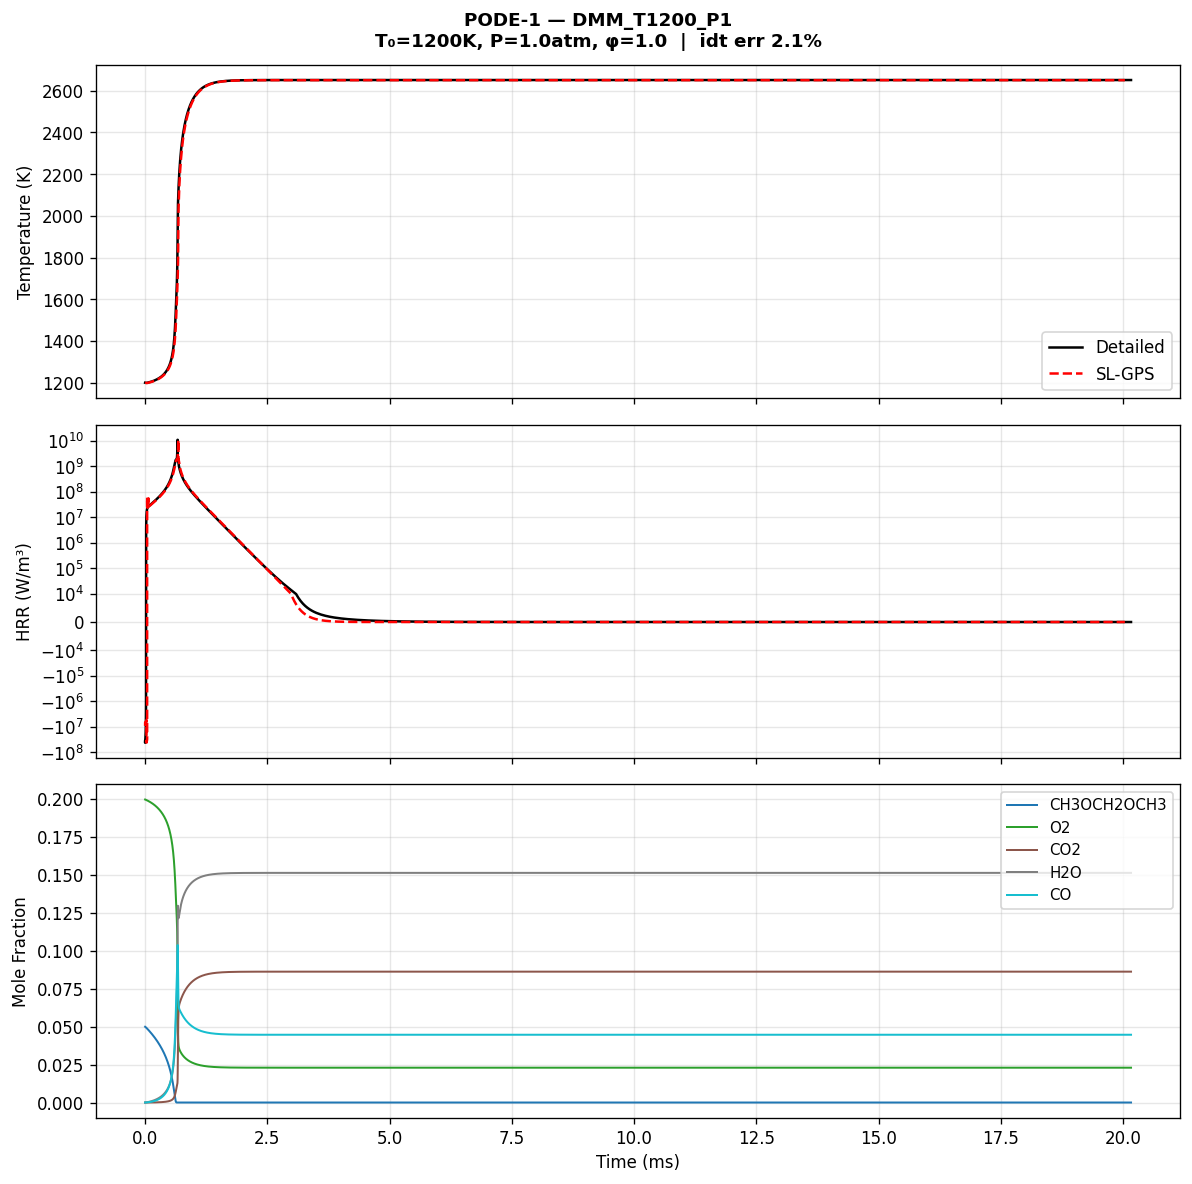
\includegraphics[width=0.95\textwidth]{results/dmm/DMM_T1200_P1.png}
    \caption{DMM: $T_0=1200$~K, $P=1$~atm, $\phi=1.0$. Ignition delay error: 2.1\%.}
\end{figure}

\begin{figure}[H]
    \centering
    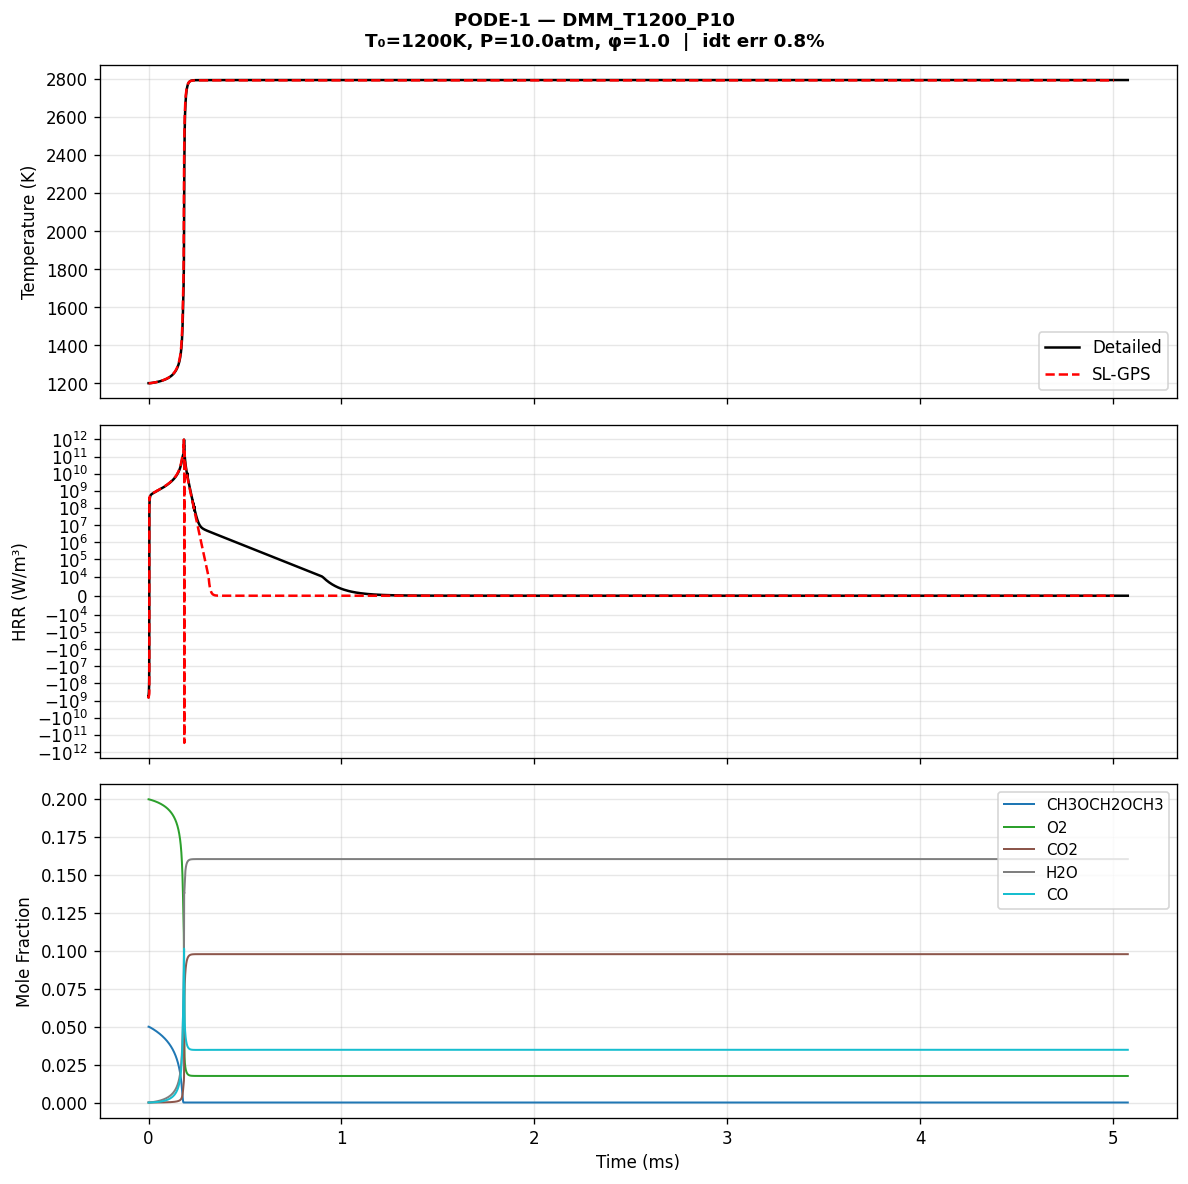
\includegraphics[width=0.95\textwidth]{results/dmm/DMM_T1200_P10.png}
    \caption{DMM: $T_0=1200$~K, $P=10$~atm, $\phi=1.0$. Ignition delay error: 0.8\%.}
\end{figure}

\begin{figure}[H]
    \centering
    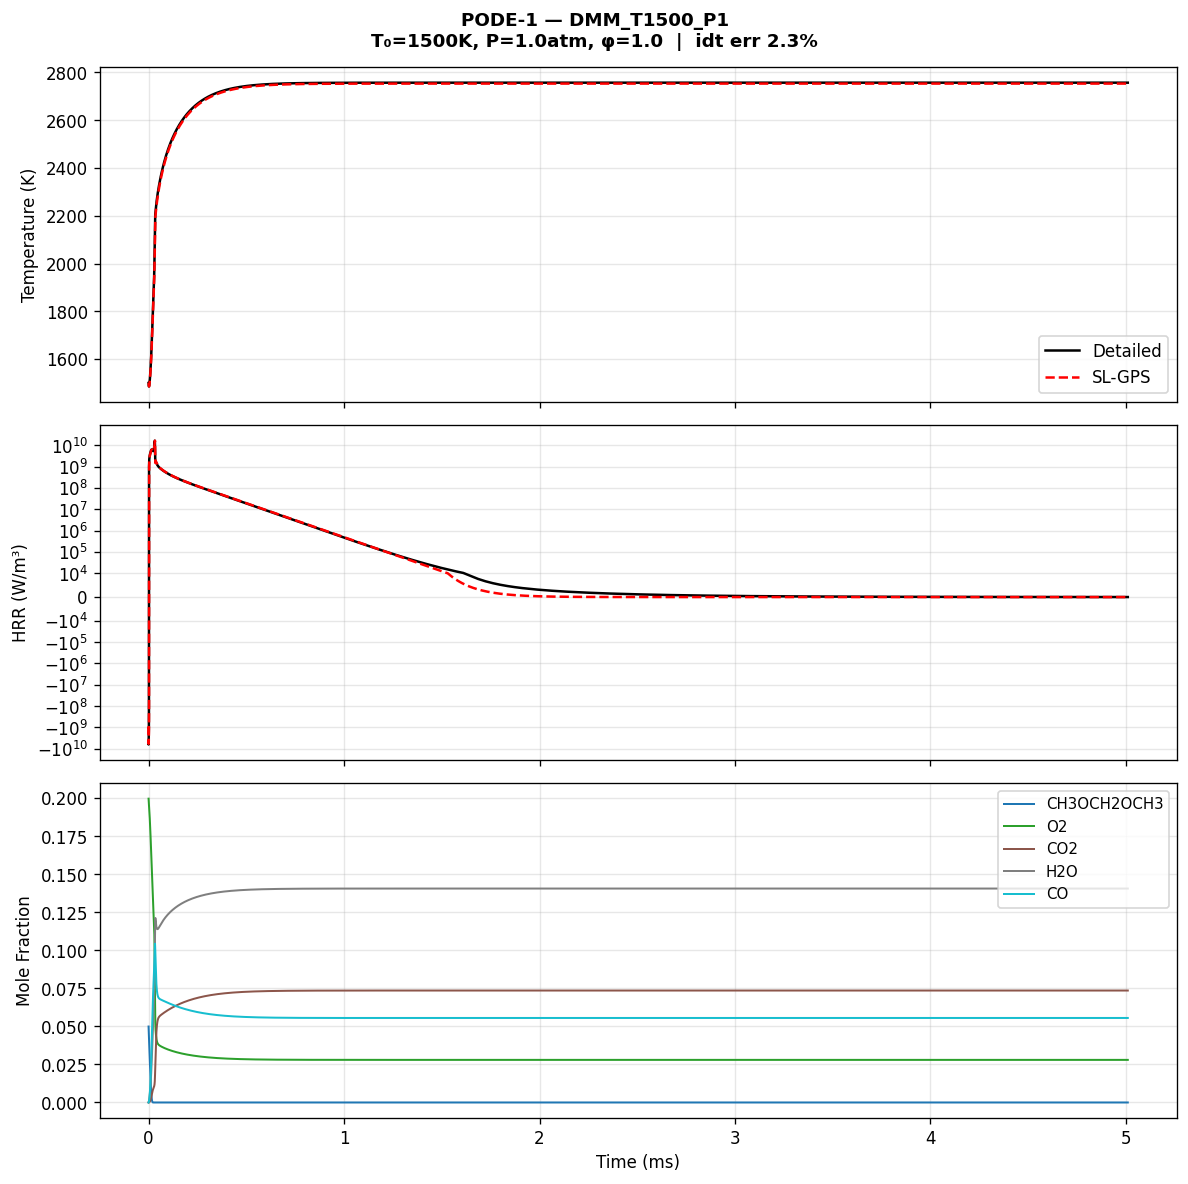
\includegraphics[width=0.95\textwidth]{results/dmm/DMM_T1500_P1.png}
    \caption{DMM: $T_0=1500$~K, $P=1$~atm, $\phi=1.0$. Ignition delay error: 2.3\%.}
\end{figure}

\begin{figure}[H]
    \centering
    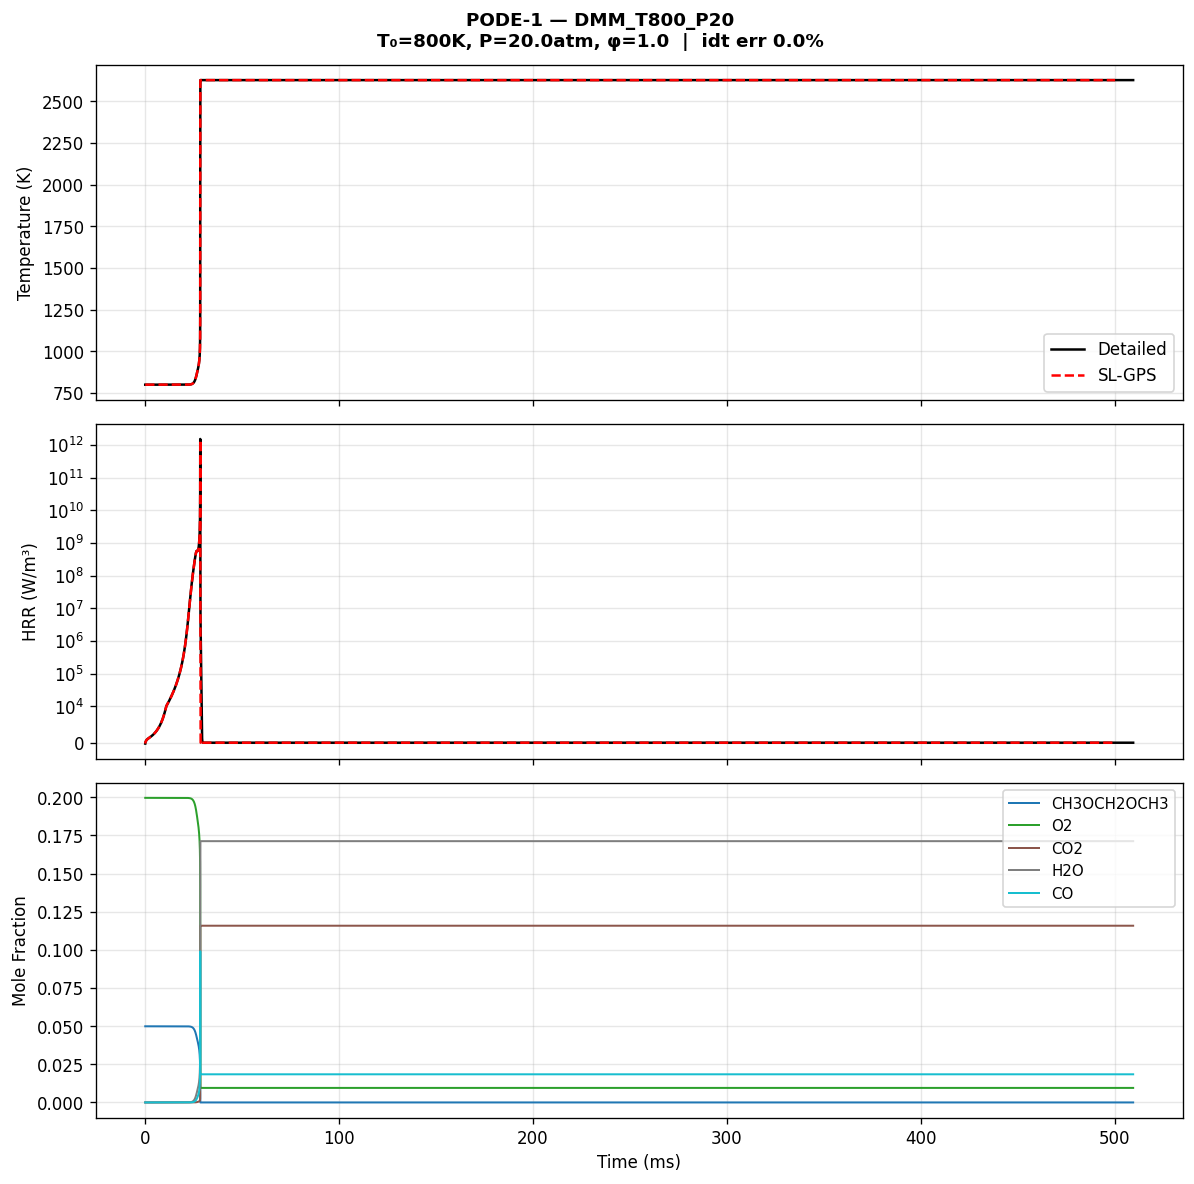
\includegraphics[width=0.95\textwidth]{results/dmm/DMM_T800_P20.png}
    \caption{DMM: $T_0=800$~K, $P=20$~atm, $\phi=1.0$ (low-T, high-P). Ignition delay error: 0.0\%.}
\end{figure}

\begin{figure}[H]
    \centering
    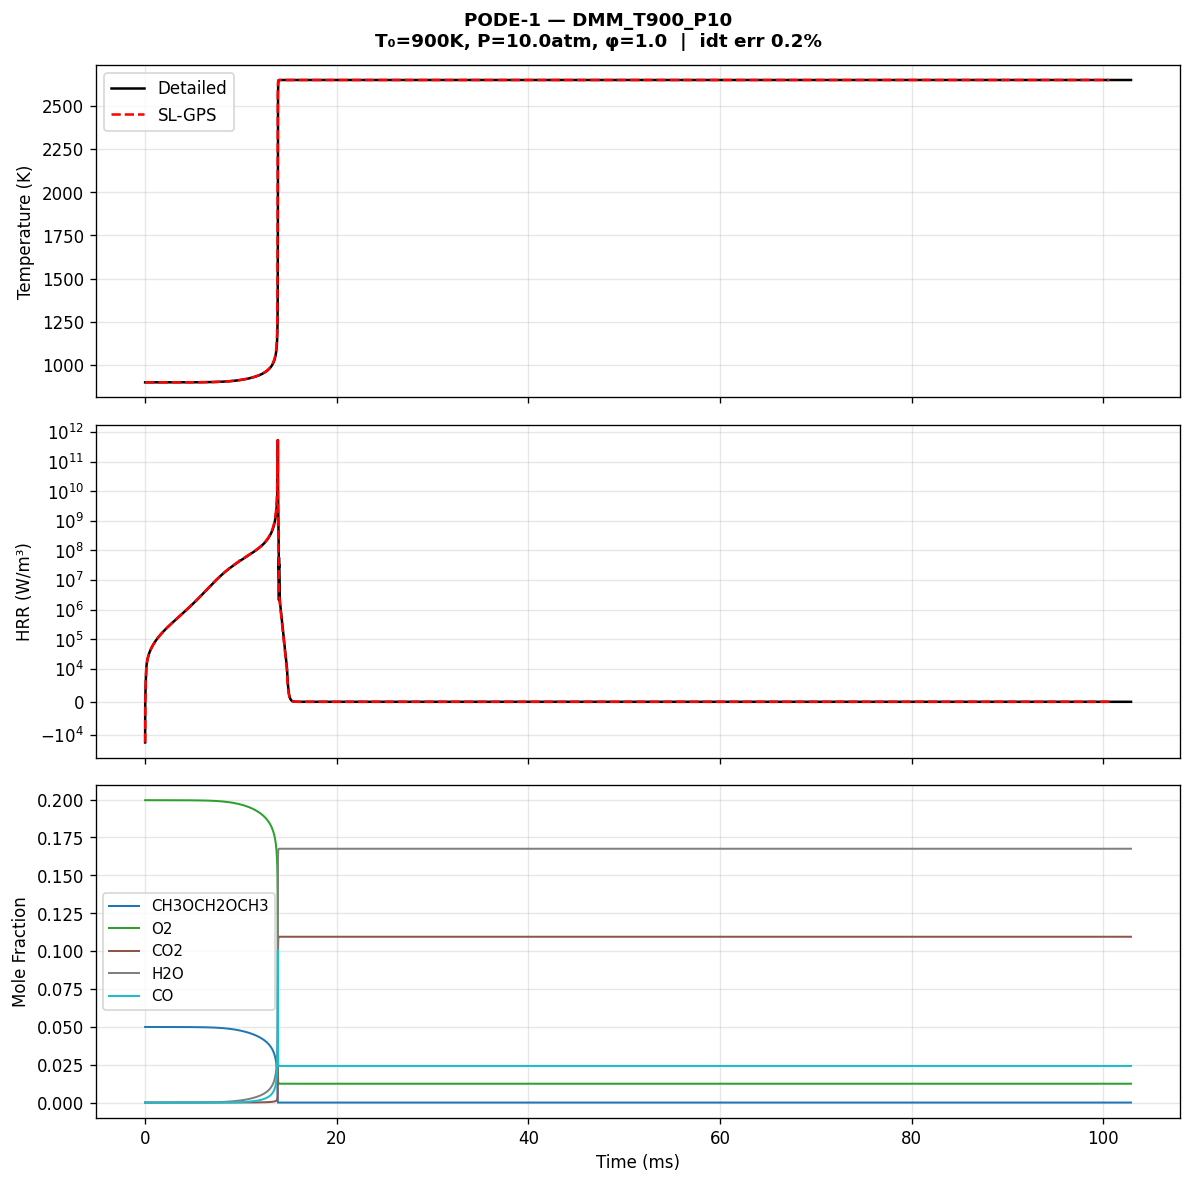
\includegraphics[width=0.95\textwidth]{results/dmm/DMM_T900_P10.png}
    \caption{DMM: $T_0=900$~K, $P=10$~atm, $\phi=1.0$ (NTC region). Ignition delay error: 0.2\%.}
\end{figure}

\begin{figure}[H]
    \centering
    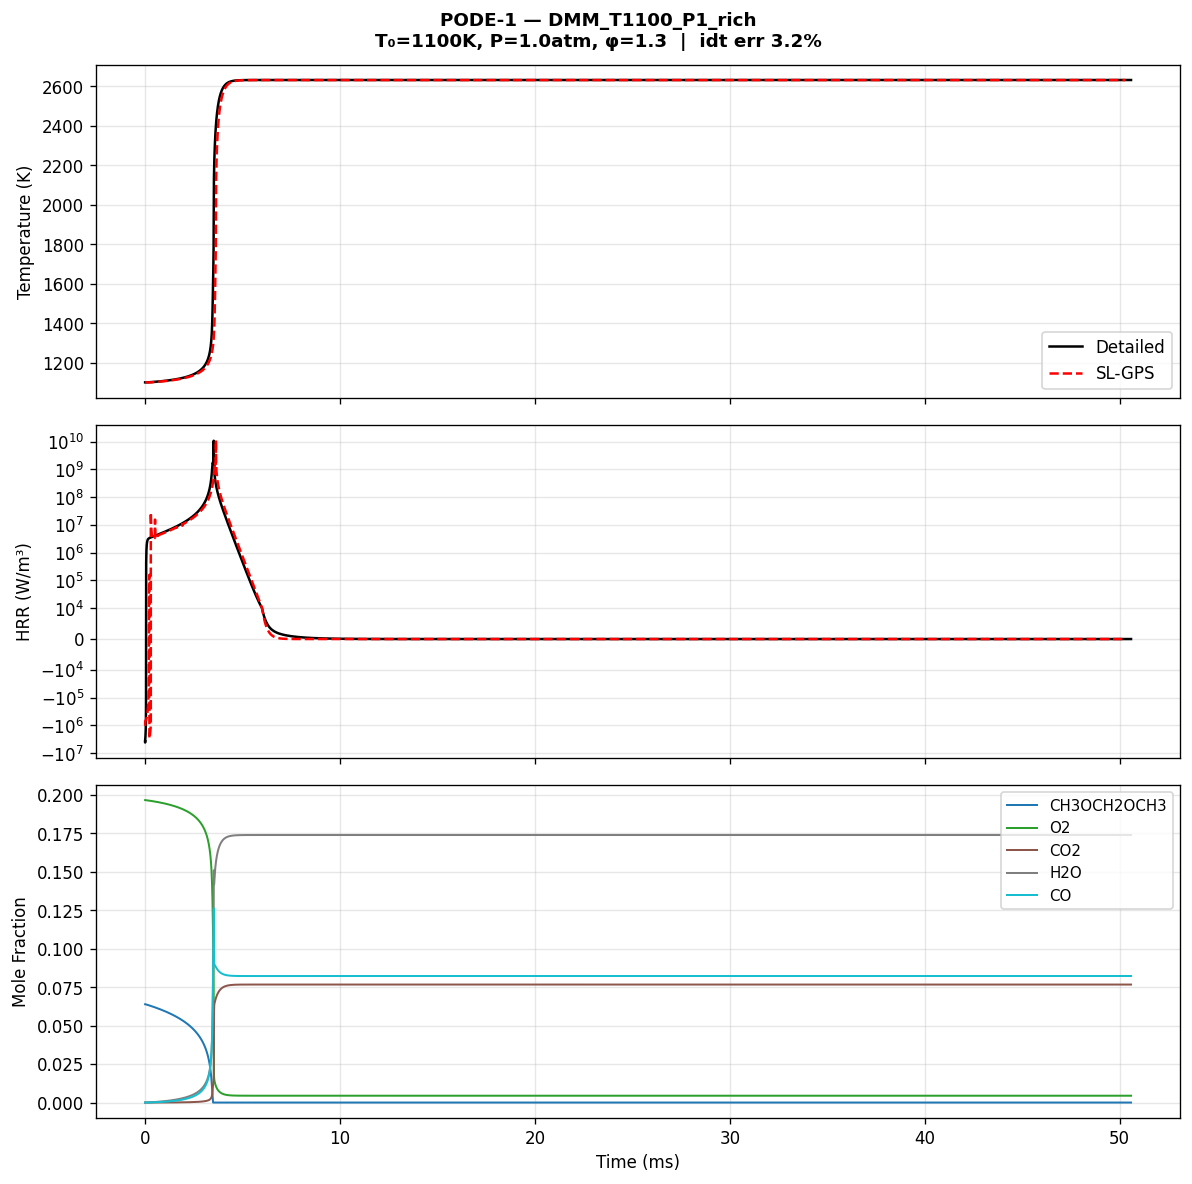
\includegraphics[width=0.95\textwidth]{results/dmm/DMM_T1100_P1_rich.png}
    \caption{DMM: $T_0=1100$~K, $P=1$~atm, $\phi=1.3$ (fuel-rich). Ignition delay error: 3.2\%.}
\end{figure}

\begin{figure}[H]
    \centering
    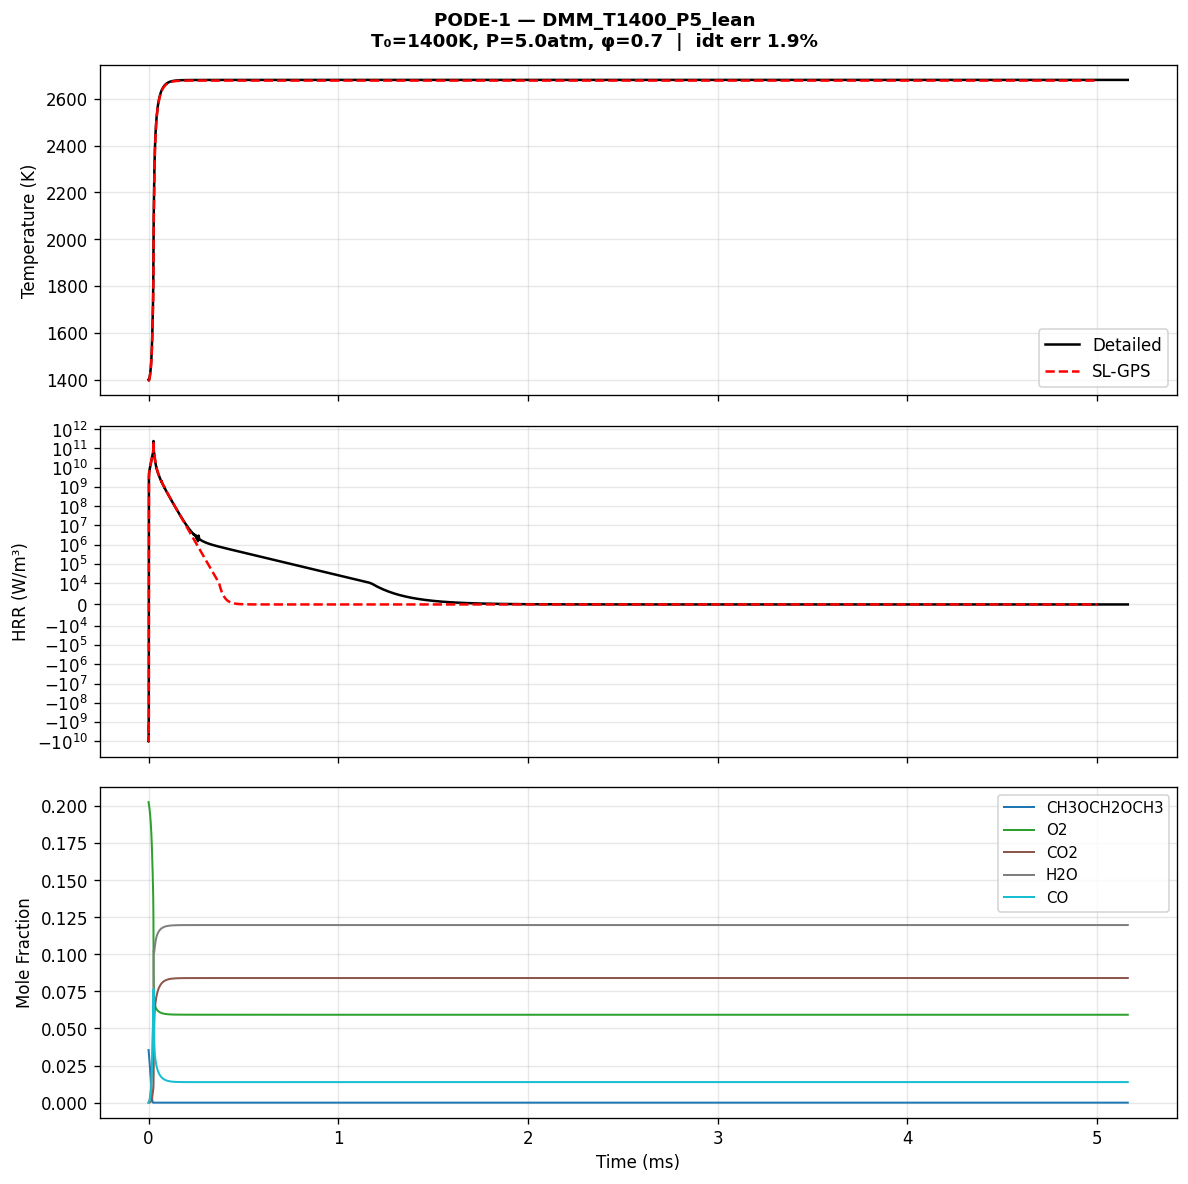
\includegraphics[width=0.95\textwidth]{results/dmm/DMM_T1400_P5_lean.png}
    \caption{DMM: $T_0=1400$~K, $P=5$~atm, $\phi=0.7$ (fuel-lean). Ignition delay error: 1.9\%.}
\end{figure}

\section{Conclusions}

The SL-GPS method has been validated on the PODE-1 mechanism (586 species, 3091 reactions) for dimethoxymethane (DMM) combustion. Key findings:

\begin{itemize}
    \item \textbf{8/8 cases pass} ($<10\%$ ignition delay error) across 800--1500~K, 1--20~atm, and $\phi=0.7$--1.3.
    \item \textbf{Mean ignition delay error: 1.4\%}, with maximum 3.2\% (fuel-rich case).
    \item \textbf{95\% mean mechanism reduction}: only 32 of 586 species active on average.
    \item Low-temperature (NTC) cases at 800--900~K show sub-0.3\% error, demonstrating robust performance.
    \item Both lean ($\phi=0.7$) and rich ($\phi=1.3$) mixtures are well captured.
\end{itemize}

These results demonstrate that SL-GPS scales effectively to large mechanisms ($>500$ species) while maintaining high accuracy and achieving dramatic mechanism reduction.

\end{document}
